%
% The first command in your LaTeX source must be the \documentclass command.
% \documentclass[acmtog]{acmart}
\documentclass[sigchi]{acmart}
\settopmatter{printacmref=false}
\settopmatter{printacmref=false}
\setcopyright{none}
\settopmatter{printacmref=false} % Removes citation information below abstract
\renewcommand\footnotetextcopyrightpermission[1]{} % removes footnote with conference information in first column
\pagestyle{plain} % removes running headers
\renewcommand\footnotetextcopyrightpermission[1]{}

\usepackage{color}
\usepackage[usenames,dvipsnames,svgnames,table]{xcolor}
%
% defining the \BibTeX command - from Oren Patashnik's original BibTeX documentation.
% \def\BibTeX{{\rm B\kern-.05em{\sc i\kern-.025em b}\kern-.08emT\kern-.1667em\lower.7ex\hbox{E}\kern-.125emX}}
%
% The majority of ACM publications use numbered citations and references. If you are preparing content for an event
% sponsored by ACM SIGGRAPH, you must use the "author year" style of citations and references. Uncommenting
% the next command will enable that style.
%\citestyle{acmauthoryear}
%
% end of the preamble, start of the body of the document source.

\begin{document}

%
% The "title" command has an optional parameter, allowing the author to define a "short title" to be used in page headers.
\title{    
	Project 2: Continuous Control\\
	{\large Udacity Deep Reinforcement Learning Nanodegree Program}
}

%
% The "author" command and its associated commands are used to define the authors and their affiliations.
% Of note is the shared affiliation of the first two authors, and the "authornote" and "authornotemark" commands
% used to denote shared contribution to the research.
\author{Bob Flagg}\affiliation{}

%
% By default, the full list of authors will be used in the page headers. Often, this list is too long, and will overlap
% other information printed in the page headers. This command allows the author to define a more concise list
% of authors' names for this purpose.
\renewcommand{\shortauthors}{Bob Flagg}

%
% The abstract is a short summary of the work to be presented in the article.

%
% The code below is generated by the tool at http://dl.acm.org/ccs.cfm.
% Please copy and paste the code instead of the example below.
%

%
% A "teaser" image appears between the author and affiliation information and the body 
% of the document, and typically spans the page. 
\begin{teaserfigure}
	\centering
  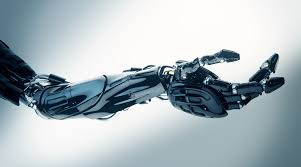
\includegraphics[width=0.4\textwidth]{arm}
  \caption{Designing a robotic arm. Source: SOLIDWORKS 2016~\protect\cite{10.1007/978-3-319-52941-7_18}}
  \label{fig:teaser}
\end{teaserfigure}

%
% This command processes the author and affiliation and title information and builds
% the first part of the formatted document.
\maketitle

%%%%%%%%%%%%%%%%%%%%%%%%%%%%%%%%%%%%%%%%%%%%%%%%%%%%%%%%%%%%%%
%% Introduction                                                                                                                             %%
%%%%%%%%%%%%%%%%%%%%%%%%%%%%%%%%%%%%%%%%%%%%%%%%%%%%%%%%%%%%%%
\section{Introduction}

In this project I'll implement a solution to the 
\href{https://github.com/Unity-Technologies/ml-agents/blob/master/docs/Learning-Environment-Examples.md#reacher}{\underline{Reacher}}
environment from the 
\href{https://unity3d.ai}{\underline{Unity Machine Learning Toolkit}}.
The Reacher is a double-jointed arm that can move to target locations. A reward of +0.1 is provided for each step 
that the agent's hand is in the goal location. Thus, the goal for the agent is to maintain its position at the target location for as many time steps as possible.

The observation space consists of 33 variables corresponding to position, rotation, velocity, and angular velocities of the arm. Each action is a vector with four numbers, corresponding to torque applicable to two joints. Every entry in the action vector should be a number between -1 and 1.


I'll use {\em Deep Deterministic Policy Gradient}~\cite{Silver:2014:DPG:3044805.3044850} (DDPG) to solve the distributed version of the task which contains 20 identical agents, each with its own copy of the environment.
Source code in Python, using PyTorch, is available on 
\href{http://github.com}{\underline{github}} 
in the repo 
\href{https://github.com/bobflagg/Continuous-Control}{\underline{Continuous-Control}}.





\section{Background}

The 
\href{https://github.com/Unity-Technologies/ml-agents/blob/master/docs/Learning-Environment-Examples.md#reacher}{\underline{Reacher}}
is a {\em sequential decision making problem}, in which an agent interacts with an environment over discrete time
steps and tries to find a {\em policy} to maximize the expected {\em discounted return}:
$$G_t = \sum_{\tau=t}^{\infty}\gamma^{\tau-t}R_\tau,$$
where $\gamma\in[0,1]$  is a discount factor that trades-off the importance of immediate and future rewards.
See~\cite{DBLP:books/lib/SuttonB98} for a general discussion of this sort of problem. 

%%%%%%%%%%%%%%%%%%%%%%%%%%%%%%%%%%%%%%%%%%%%%%%%%%%%%%%%%%%%%%
%% Deep Q-Learning for Navigation                                                                                                %%
%%%%%%%%%%%%%%%%%%%%%%%%%%%%%%%%%%%%%%%%%%%%%%%%%%%%%%%%%%%%%%
\section{Soft Actor-Critic}

\subsection{Entropy-Regularized Reinforcement Learning}

$$\pi^* =  \operatorname{arg\,max}_{\pi}\mathbb{E}_{\tau\sim\pi}\big[\sum_{t=0}^{\infty}\gamma^t\big(R_t+\alpha \mathcal{H} [\pi(\cdot|S_t)]\big)\big].$$

$$L(\phi_i, {\mathcal D}) = \underset{(s,a,r,s',d) \sim {\mathcal D}}{\mathbb{E}}\left[
\Bigg( Q_{\phi_i}(s,a) - \left(r + \gamma (1 - d) V_{\psi_{\text{targ}}}(s') \right) \Bigg)^2
\right].$$

\begin{enumerate}
	\item\textbf{Near Duplicate N-Grams}: We'll maintain a database of about 80,000 pre-populated ad text transcript n-gram hashes (updated on a regular basis) and a dynamic collection of hashes collected from repeated content determined to be ad text and use this database to extract the following features of a segment:
		\begin{enumerate}
			\item duplicate n-grams across programs,
			\item duplicate n-grams across station boundaries,
			\item duplicate n-grams across affiliate boundaries, and
			\item duplicate n-grams across broadcast markets.
		\end{enumerate}
	\item\textbf{Transcript Line Timing}: Line timing is likely to be predictive of advertisements and we'll consider the following features derived from it:
		\begin{enumerate}
			\item 3-4 second preceding pause,
			\item number of seconds since the top of the hour,
			\item number of seconds since the end of the last ad pod,
			\item number of seconds since the last transition,
			\item station or program specific timing of ads,
			\item time of day, and
			\item day of the week
		\end{enumerate}
\end{enumerate}


%%%%%%%%%%%%%%%%%%%%%%%%%%%%%%%%%%%%%%%%%%%%%%%%%%%%%%%%%%%%%%
%% Other Languages                                                                                                                      %%
%%%%%%%%%%%%%%%%%%%%%%%%%%%%%%%%%%%%%%%%%%%%%%%%%%%%%%%%%%%%%%
\section{Other Languages}

The APDE design outlined above can be built to support any language provided the following resources are available in the target language:

\begin{enumerate}
	\item a large (> 500K docs) corpus of program transcripts for unsupervised training of a topic model,
	\item a reasonably large (about 5K docs) collection of program transcripts with advertisement segments tagged for supervised training of a text classifier, and
	\item a resource for maintaining a database of pre-populated ad text transcript n-gram hashes.
\end{enumerate}


\bibliographystyle{ACM-Reference-Format}
\nocite{*}
\bibliography{report}


\end{document}


{\em Soft Actor-Critic Algorthm}~\cite{DBLP:journals/corr/abs-1812-05905}.
Source code in Python, using PyTorch, is available on 
\href{http://github.com}{\underline{github}} 
in the repo 
\href{https://github.com/bobflagg/Actor-Critic-for-Continuous-Control}{\underline{Actor-Critic-for-Continuous-Control}}.



%%%%%%%%%%%%%%%%%%%%%%%%%%%%%%%%%%%%%%%%%%%%%%%%%%%%%%%%%%%%%%
%% Resources                                                                                                                               %%
%%%%%%%%%%%%%%%%%%%%%%%%%%%%%%%%%%%%%%%%%%%%%%%%%%%%%%%%%%%%%%
\section{Additional Resources}

\begin{enumerate}
	
	\item \href{https://blog.lateral.io/2017/10/text-segmentation-using-word-embeddings/}{\color{red}Text Segmentation using Word Embeddings}
	\item \href{http://www.cs.man.ac.uk/~mary/choif/software.html}{\color{red}Freddy Choi: Code and data for segmentation experiments}
	\item \href{https://github.com/datafordemocracy/topictiling}{\color{red}Repository that does topictiling on cable news}
	\item \href{https://github.com/logological/C99}{\color{red}C99, a domain-independent algorithm for linear text segmentation by Freddy Choi}
	\item \href{https://github.com/levy5674/text-tiling-demo}{\color{red}Demo of ntlk's TextTilingTokenizer}
	\item \href{http://politicaladarchive.org/data/}{\color{red}Political TV Ad Archive}
	\item \href{http://classif.ai/dataset/tv-news-channel-commercial-detection-dataset/}{\color{red}TV News Channel Commercial Detection Dataset}
	\item \href{http://github.com/alexalemi/segmentation}{\color{red}Alex Alemi: Code and data for segmentation experiments}
	
\end{enumerate}


